\documentclass[11pt,a4paper]{article}

\usepackage[utf8]{inputenc}
\usepackage[english]{babel}
\usepackage[T1]{fontenc}
\usepackage{graphicx}


\usepackage{amsmath,amssymb,amsfonts}

\title{Assignment 1}
\author{Sebastian Paaske Tørholm \& Kristoffer Søholm}

\begin{document}
\maketitle

\section{Question 1.1}
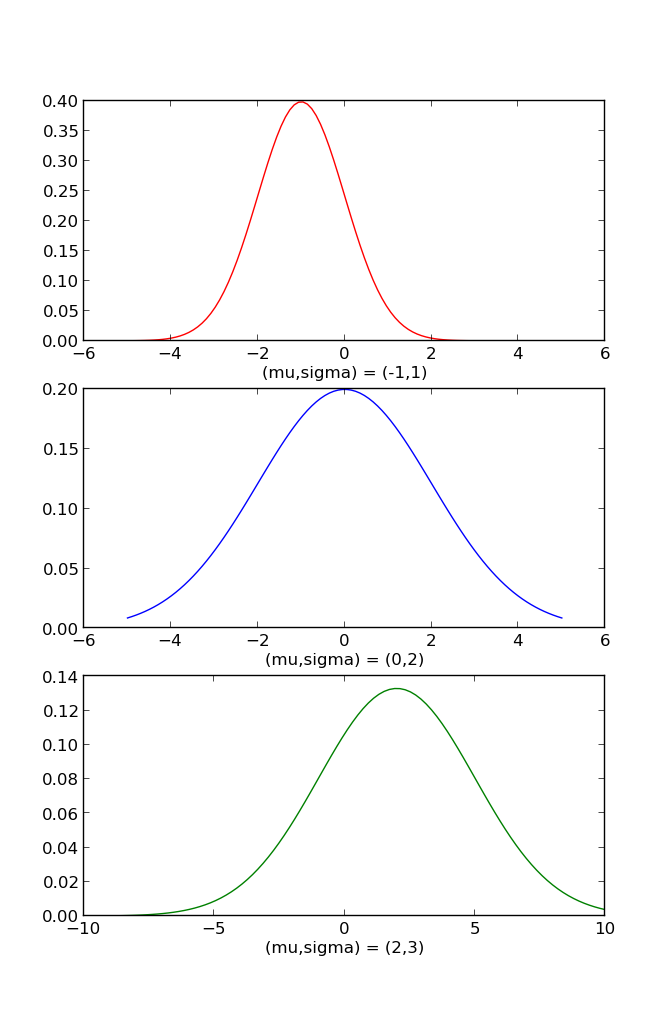
\includegraphics[width=1.1\textwidth]{figure_1.png}
\section{Question 1.2}
See the attached source.
\section{Question 1.3}
We see a deviation from the correct mean due to the values being randomly sampled. Thus it
is unlikely that we get an exact match between the sample mean and the correct mean.

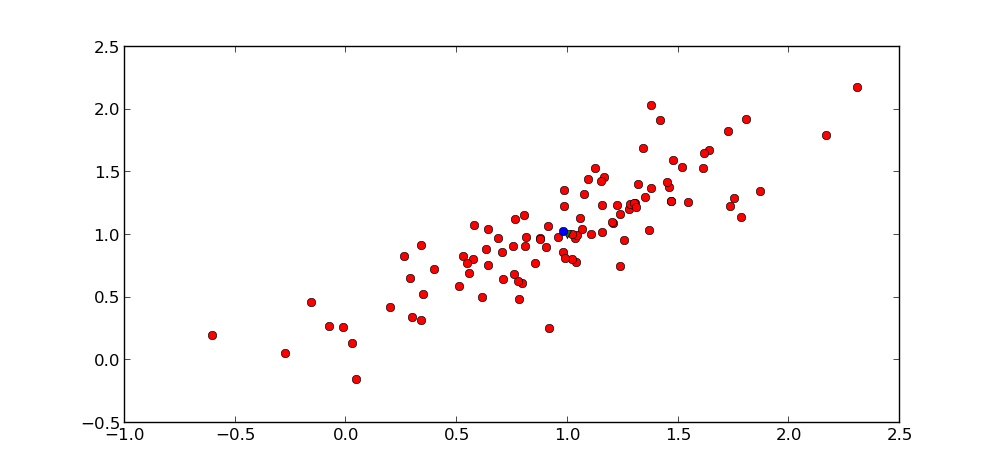
\includegraphics[width=1.1\textwidth]{figure_2.png}
\section{Question 1.4}
In order to marginalize $x_c$ out, it is sufficient to simply drop the parts of $x$, $\mu$, and $\Sigma$ which contains subscript c's. 
\section{Question 1.5}
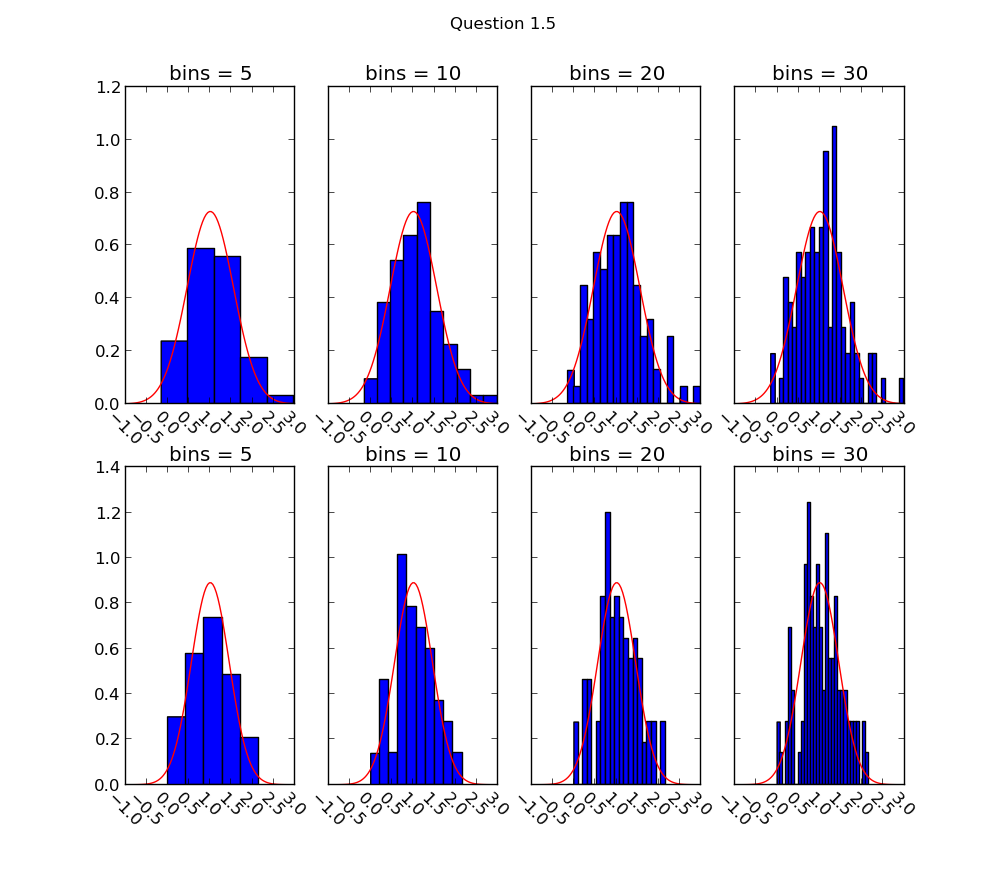
\includegraphics[width=1.1\textwidth]{figure_3.png}

Increasing the number of bins makes the histogram more accurate up to a point. As can be seen from the examples with 30 bins, the histogram becomes more erratic, as two adjacent bins get very different heights due to random fluctutations.
\section{Question 1.6}
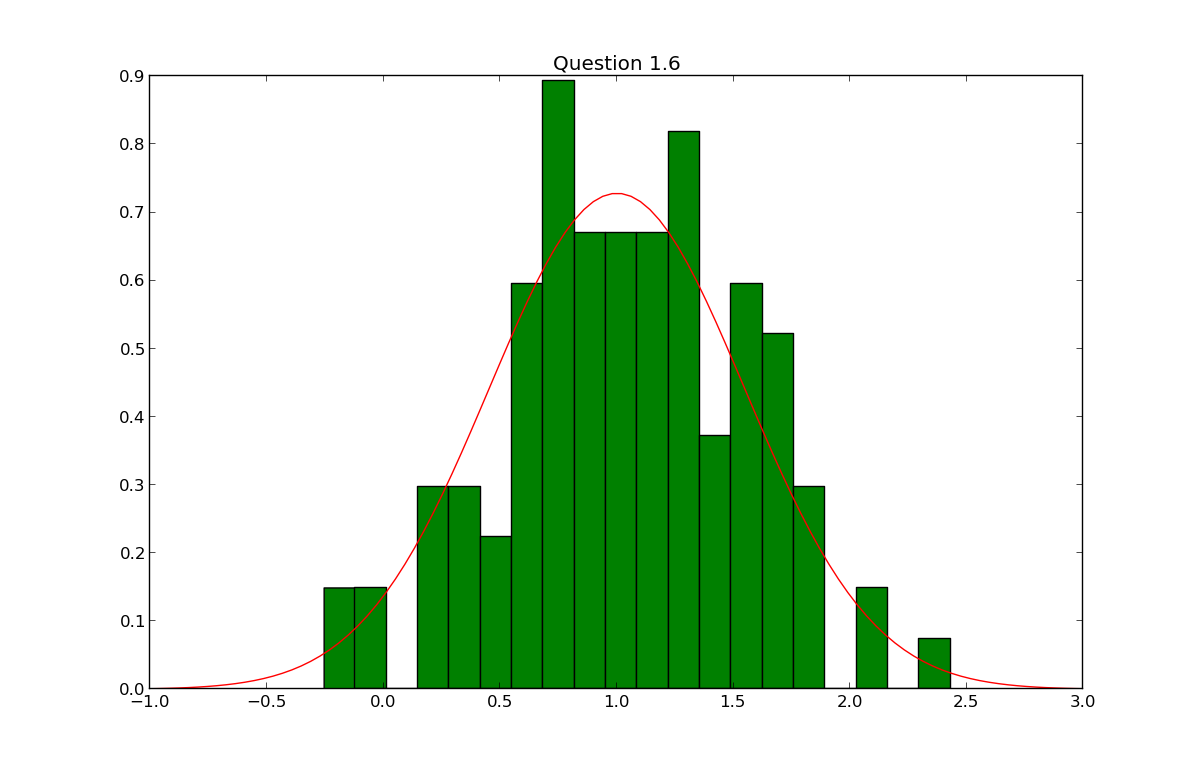
\includegraphics[width=1.1\textwidth]{figure_4.png}

The analytical expression for the marginal distribution $p(x_1)$ is given by:

$$ p(x_1) = \mathcal{N}(x_1 | 1, 0.3) $$
\section{Question 1.7}
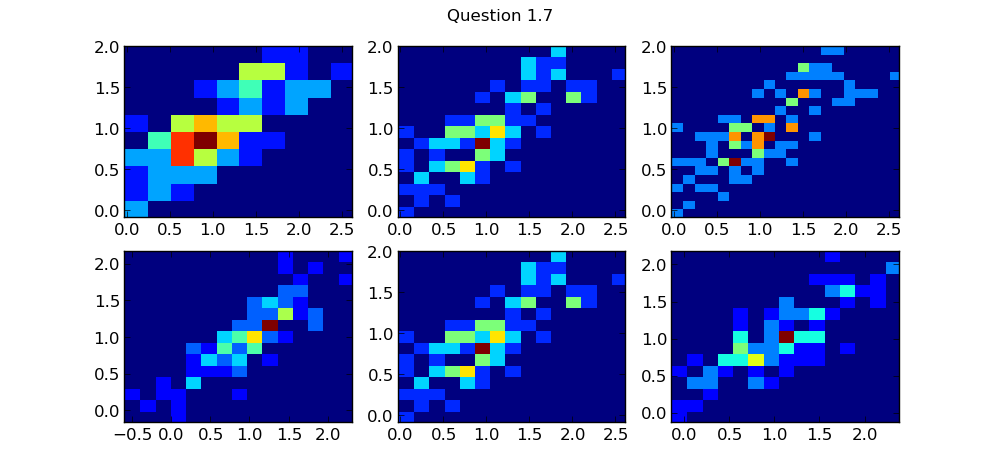
\includegraphics[width=1.1\textwidth]{figure_5.png}

In the first histogram the highest concentration lies around the expected mean $(1,1)$.
The shape of the probability densities seems to match the general form of the covariance
matrix (shown in figure 2.8 in CB), which is expected. The same problem with erratic
behaviour as in Question 1.5 is seen when the number of bins are increased with the same
amount of samples.

\section{Question 1.8}
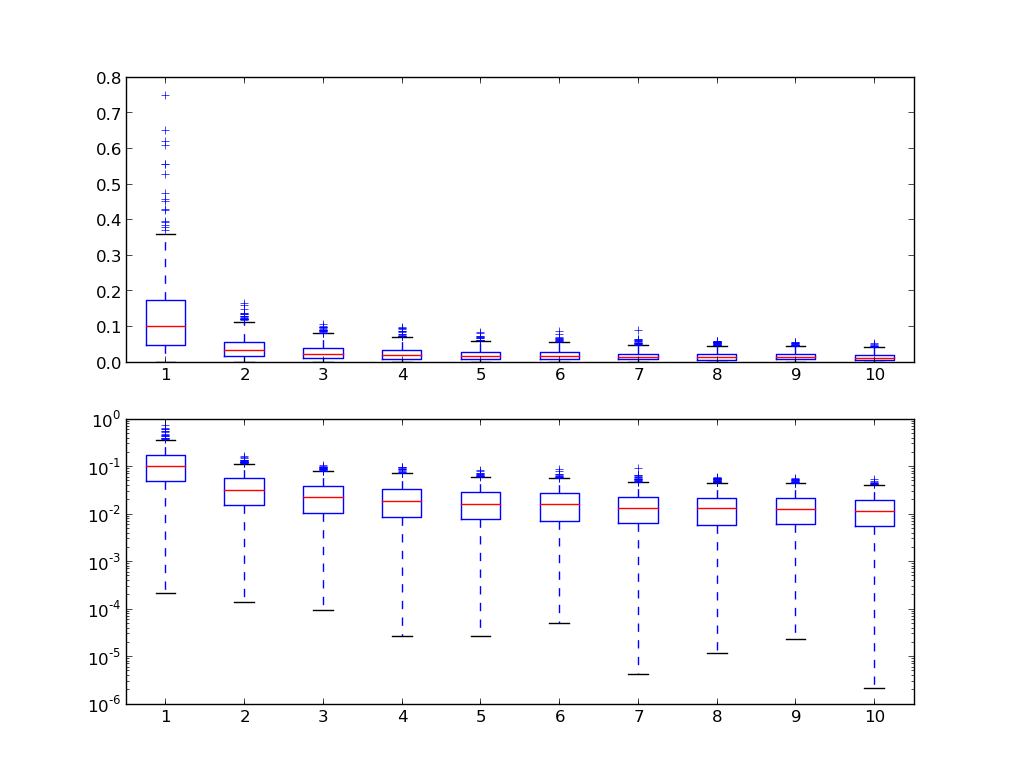
\includegraphics[width=1.1\textwidth]{figure_6.png}

The absolute devation of the exponential distribution seems to follow an exponentially decreasing curve. Huh, imagine that. This is also confirmed by the logarithmic plot below it, where the points follow a straight line.
\section{Question 1.9}
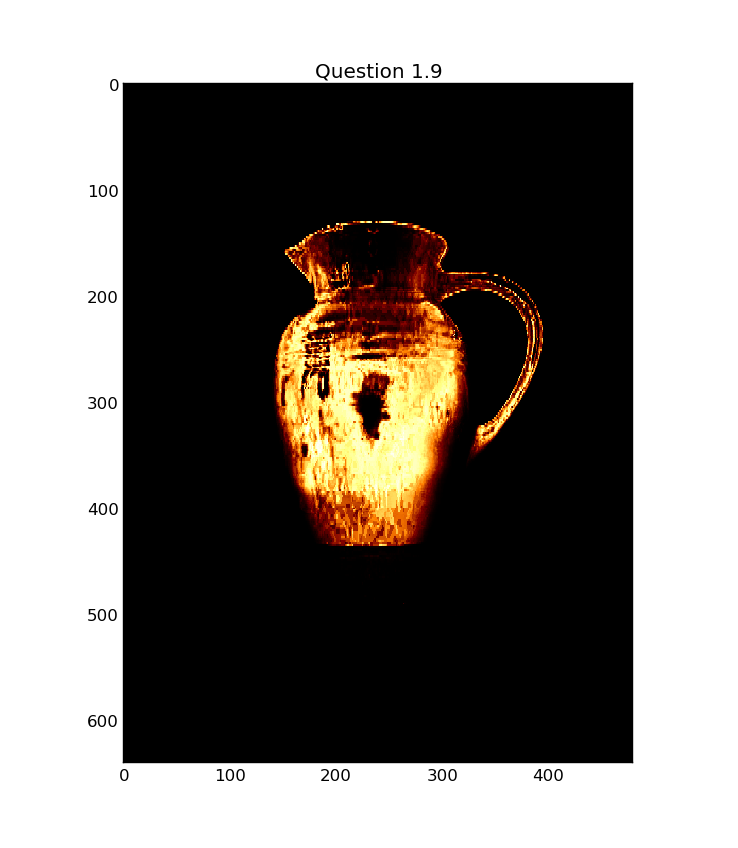
\includegraphics[width=1.1\textwidth]{figure_7.png}

The model seems to fit quite nicely on this image, which isn't too surprising given the
extensive training region and very good lighting conditions. It finds the entire pitcher
and doesn't mark anything which isn't the pitcher.


\section{Question 1.10}
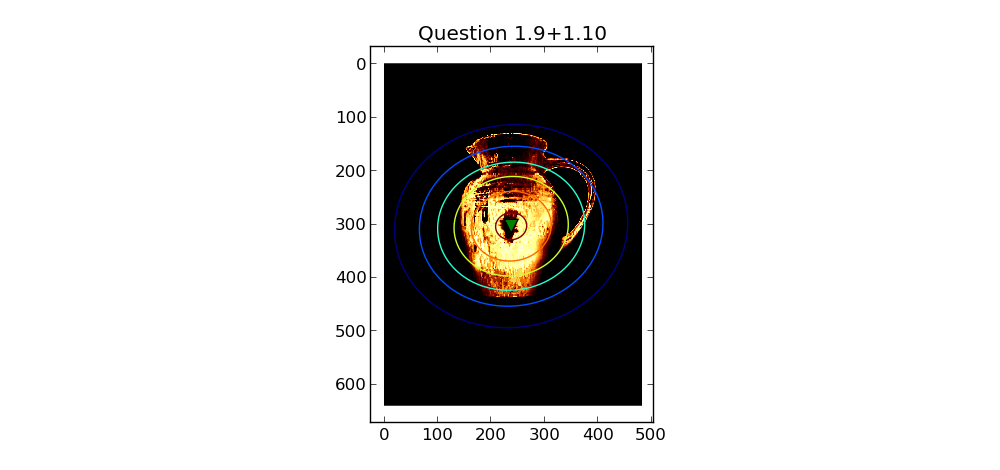
\includegraphics[width=1.1\textwidth]{figure_8.png}

The center of mass is right in the middle of the pitcher, and therefore it is a really
good estimate of the pitchers location.
\section{Question 1.11}
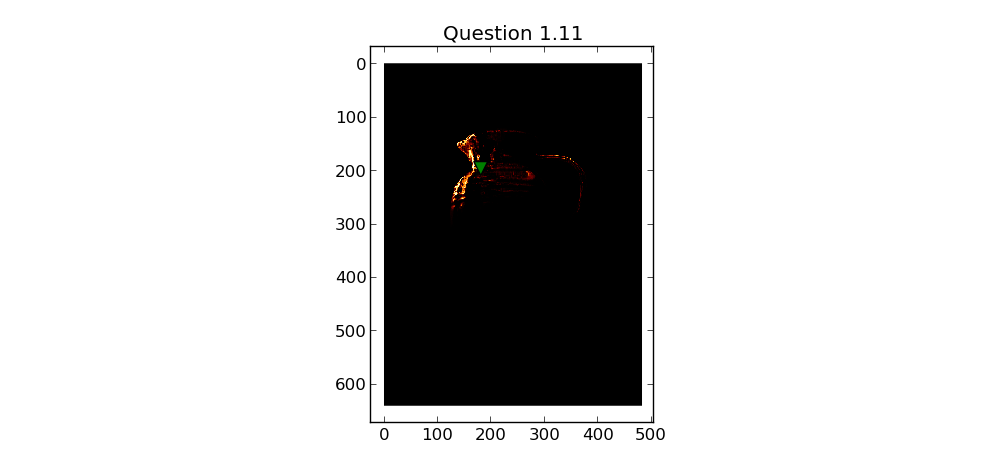
\includegraphics[width=1.1\textwidth]{figure_9.png}

We have re-used the model and training region from Question 1.9 on the other given image of the pitcher. While it doesn't find the entire pitcher, what it does find are part of the pitcher, and the center of mass is on the pitcher. As such, it can be used for detecting the location of the pitcher, although a better model will probably be needed if the lighting conditions deteriorates further.
\end{document}

